\section{Design}

\subsection{Nodes}

\subsubsection{Components}

The first step in the design process was selecting hardware components that
could operate autonomously without mains power. This required devices that were
highly power-efficient, while also capable of transmitting small data
packets via LoRa. An equally important consideration was ensuring the final
devices could be fully weatherproofed to protect the sensitive electronics from
water ingress and environmental damage.

\paragraph{Challenger RP2040 LoRa}

The iLabs Challenger RP2040 LoRa is an embedded computer that uses the Raspberry Pi
RP2040 chip that was released in 2021. The RP2040 itself is a low-cost and
power-efficient processor with ample power to perform the data encoding and
transmission in my use case. Additionally, the chip is extremely popular with
over 10 million units being produced in the first two years of release
\cite{pounder2023}. This popularity means there is ample documentation for
developing with this processor and it is compatible with circuit python which was
my preferred language for development.

\begin{figure}[H]
    \centering
    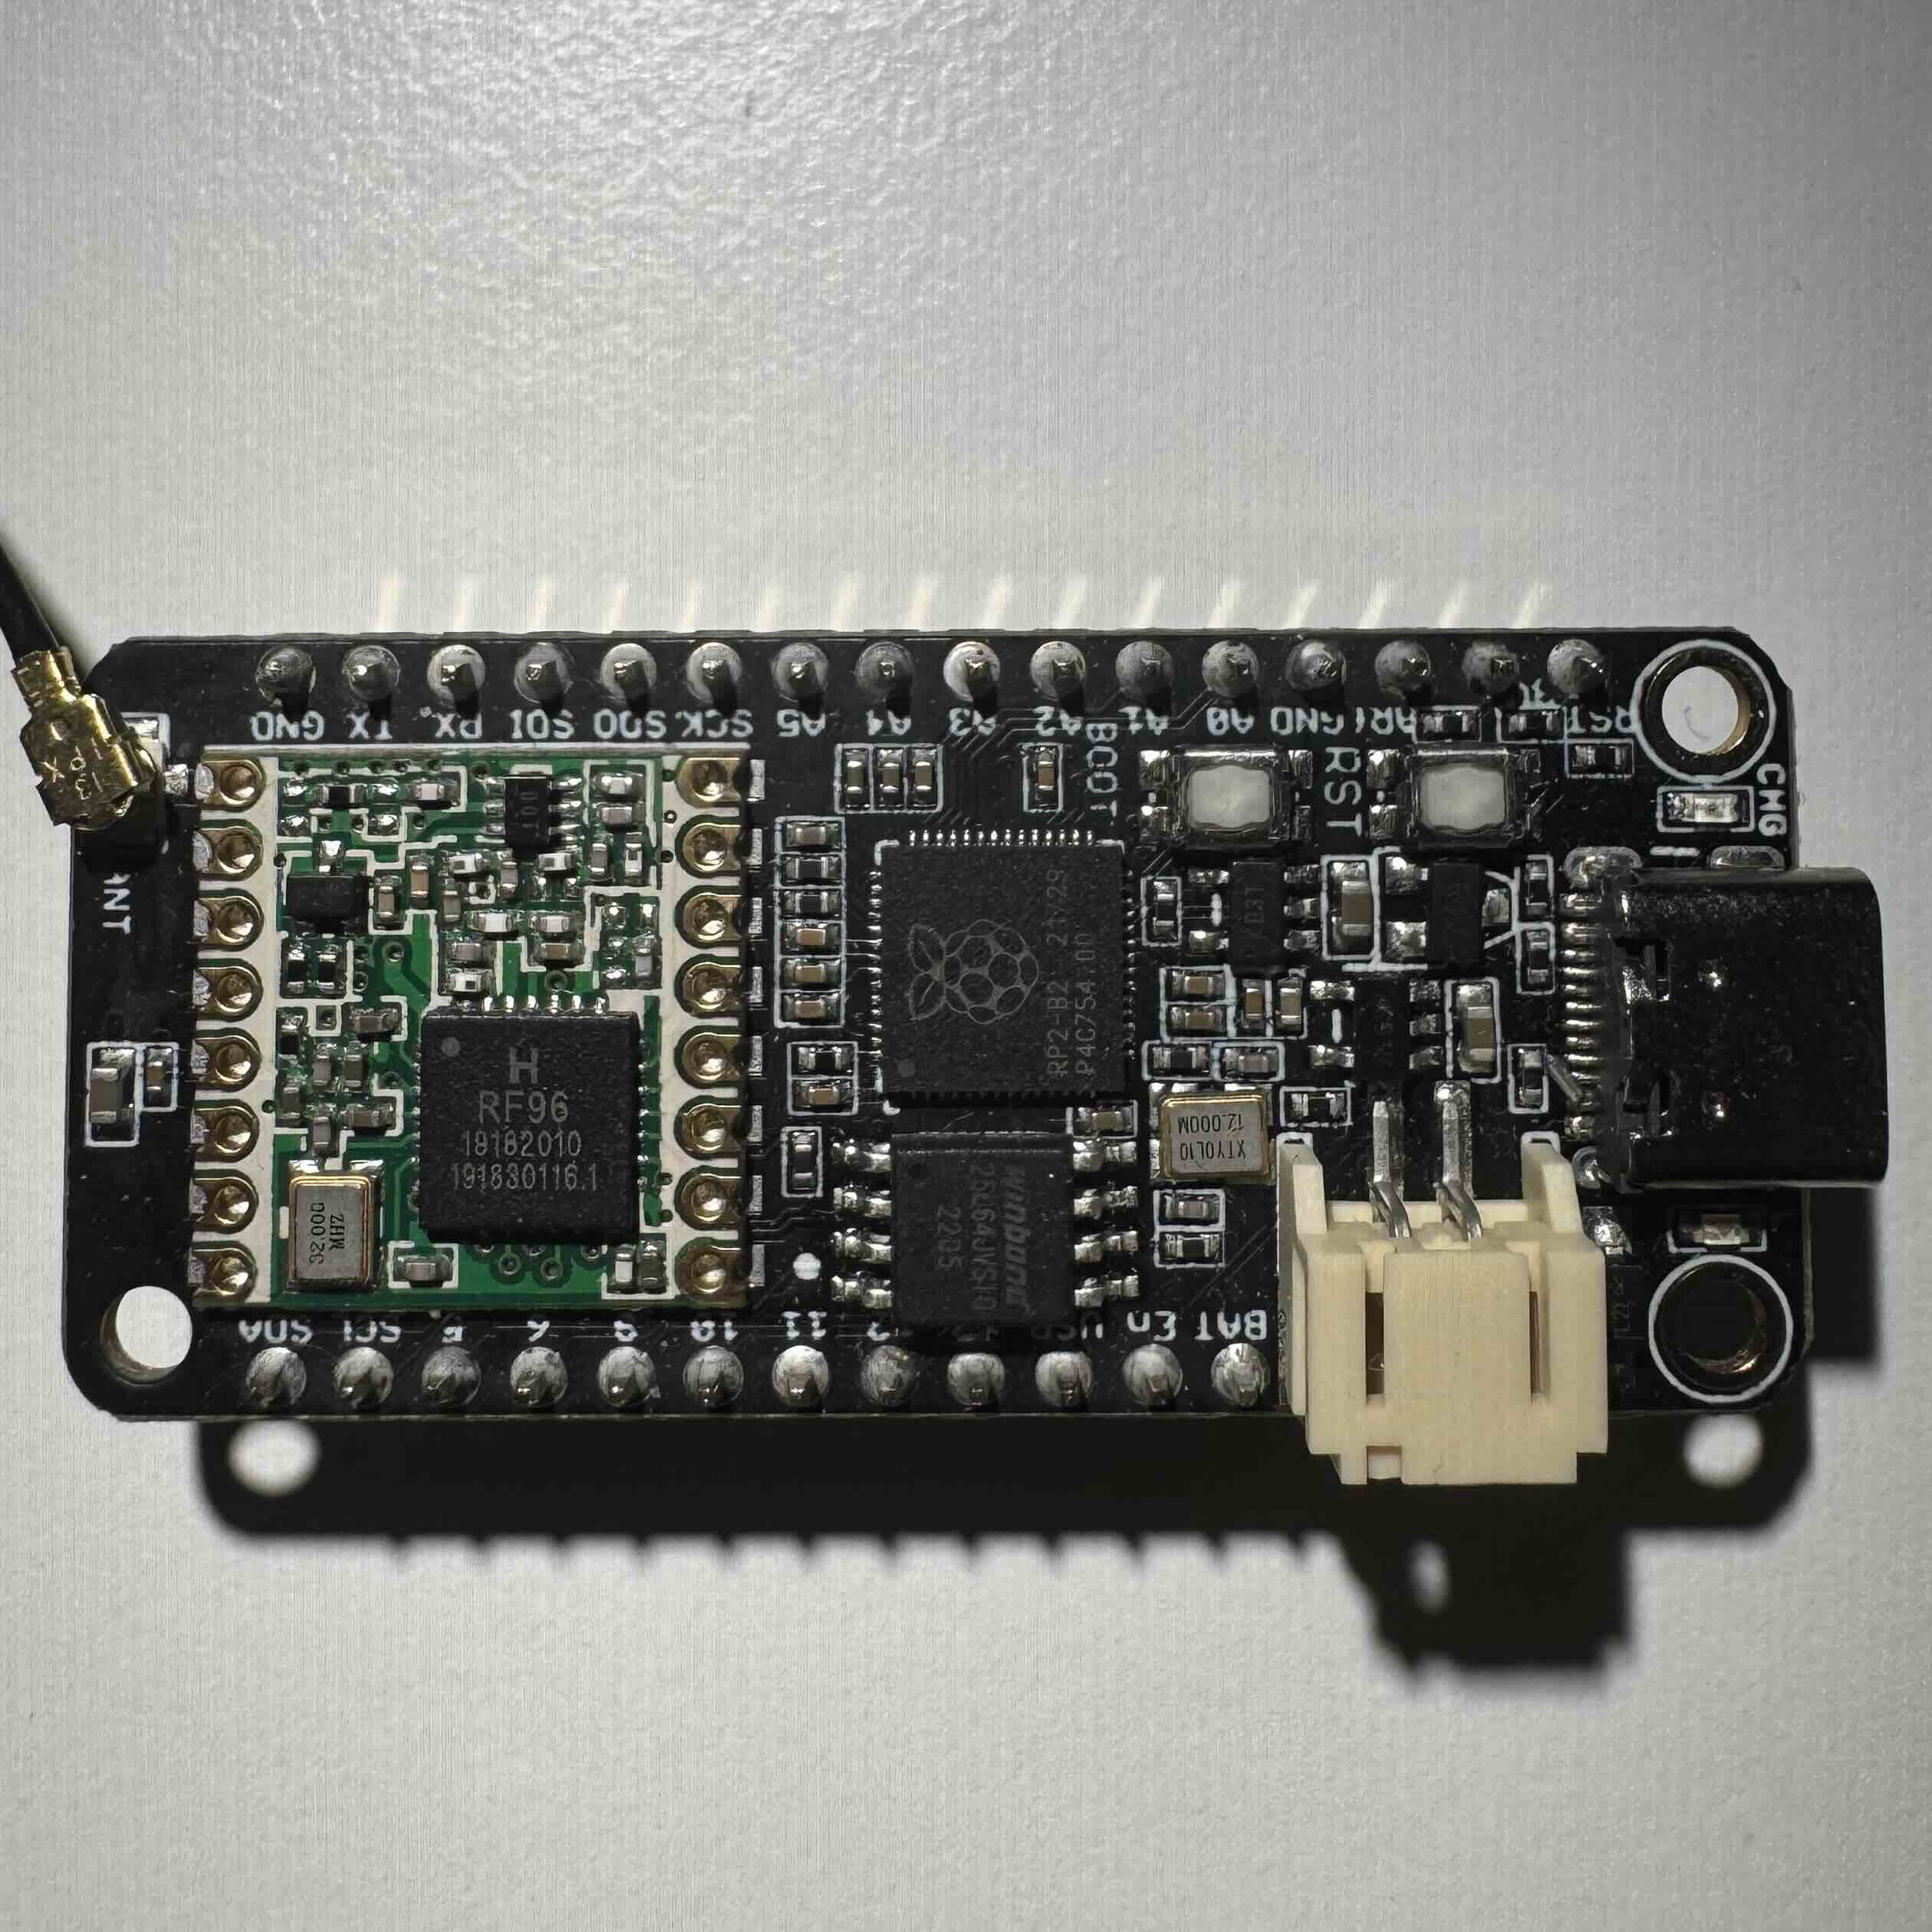
\includegraphics[width=0.9\textwidth]{contents/22-hw-design/22-fig/challenger-rp2040.jpg}
    \caption{iLabs Challenger RP2040 used in the project. Note the RP2040 chip centre and RF96 LoRa module to the right.}
    \label{fig:challenger-rp2040}
\end{figure}

The challenger board itself is well suited for this project for several reasons.
It uses the compact Adafruit feather form factor, giving a board dimension of
just 5cm by 2cm, making it easy to mount in a small enclosure. The onboard Hope
RF96 LoRa modem is built directly into the board and the U.FL antenna connector
allows for the swapping of antenna's to different varieties. This board's LoRa
module is also set to transmit at a frequency of 868mhz which is a standard UK
frequency for LoRa and gives a good balance between range and bandwidth. 

Another useful aspect of the board is the abundance of GPIO pins (20 in total)
allowing for a large number of sensors to be fitted to the board. 

\paragraph{Antennae}

The selection of antennae is one of the largest determinants of range and
reliability in the context of wireless communication systems \cite{khan2016}.
Initially I used a simple PCB antenna as shown in Figure~\ref{fig:pcb-antenna},
however as explained in the next chapter, the range of this was insufficient for
my use. 

\begin{figure}[H]
    \centering
    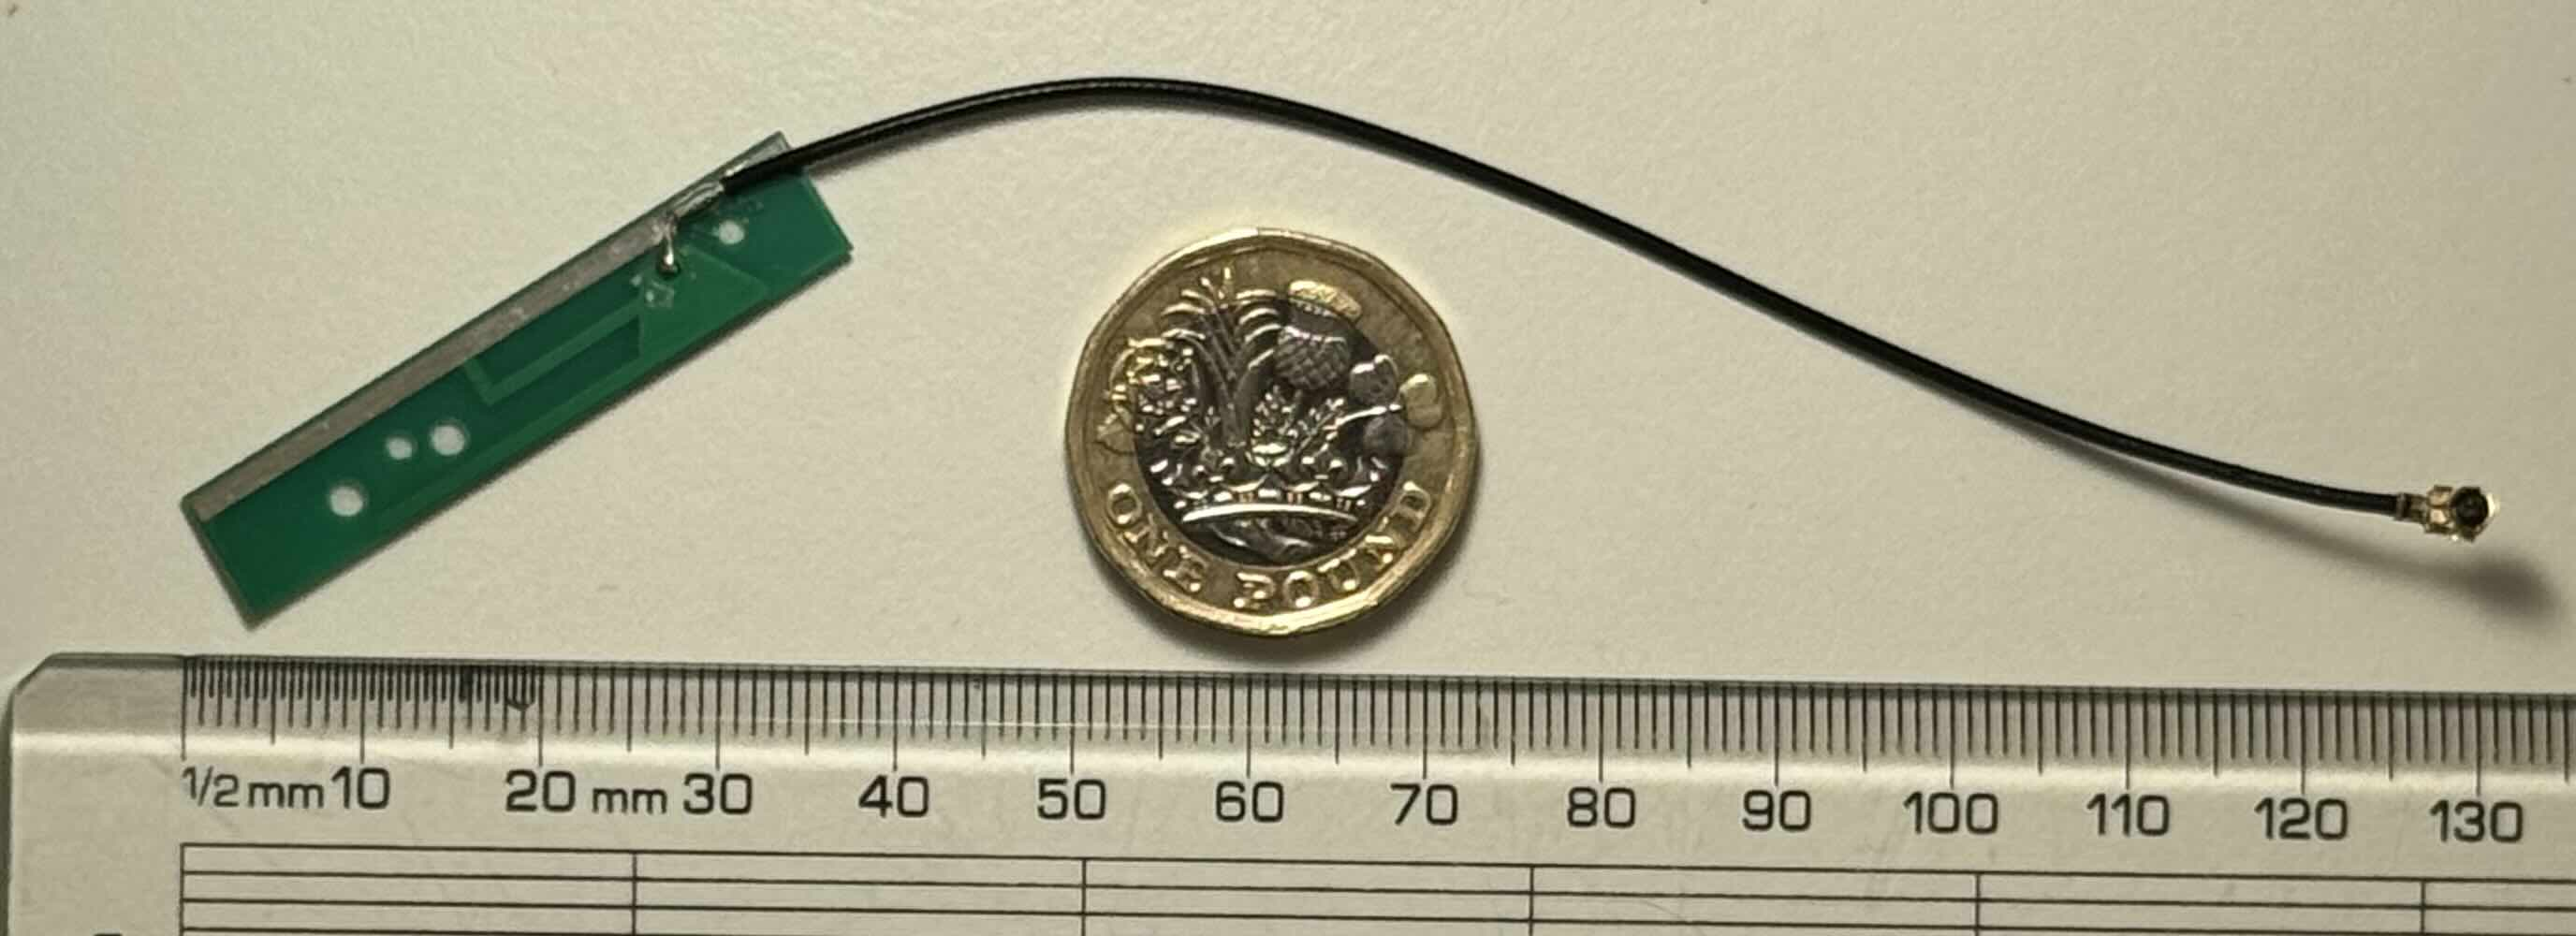
\includegraphics[width=0.9\textwidth]{contents/22-hw-design/22-fig/basic-antenna.jpg}
    \caption{Low range PCB antenna}
    \label{fig:pcb-antenna}
\end{figure}

To improve overall range I switched to a more capable 170mm whip style antenna
kit that was made specifically for the Challenger RP2040. The antenna tuned to
perform best at the 868mhz frequency range - which is the range I was using.

\paragraph{Sensor selection}

\subparagraph{Temperature and humidity sensor}

I used a DHT11 temperature/humidity sensor for each node to provide basic
readings. It was chosen for it's low cost, availability and compatibility with
both the RP2040 Challenger and CircuitPython (via libraries). The sensor can be
connected to the microcontroller using a single GPIO pin as well as the usual
power and ground pin.

\begin{figure}[H]
    \centering
    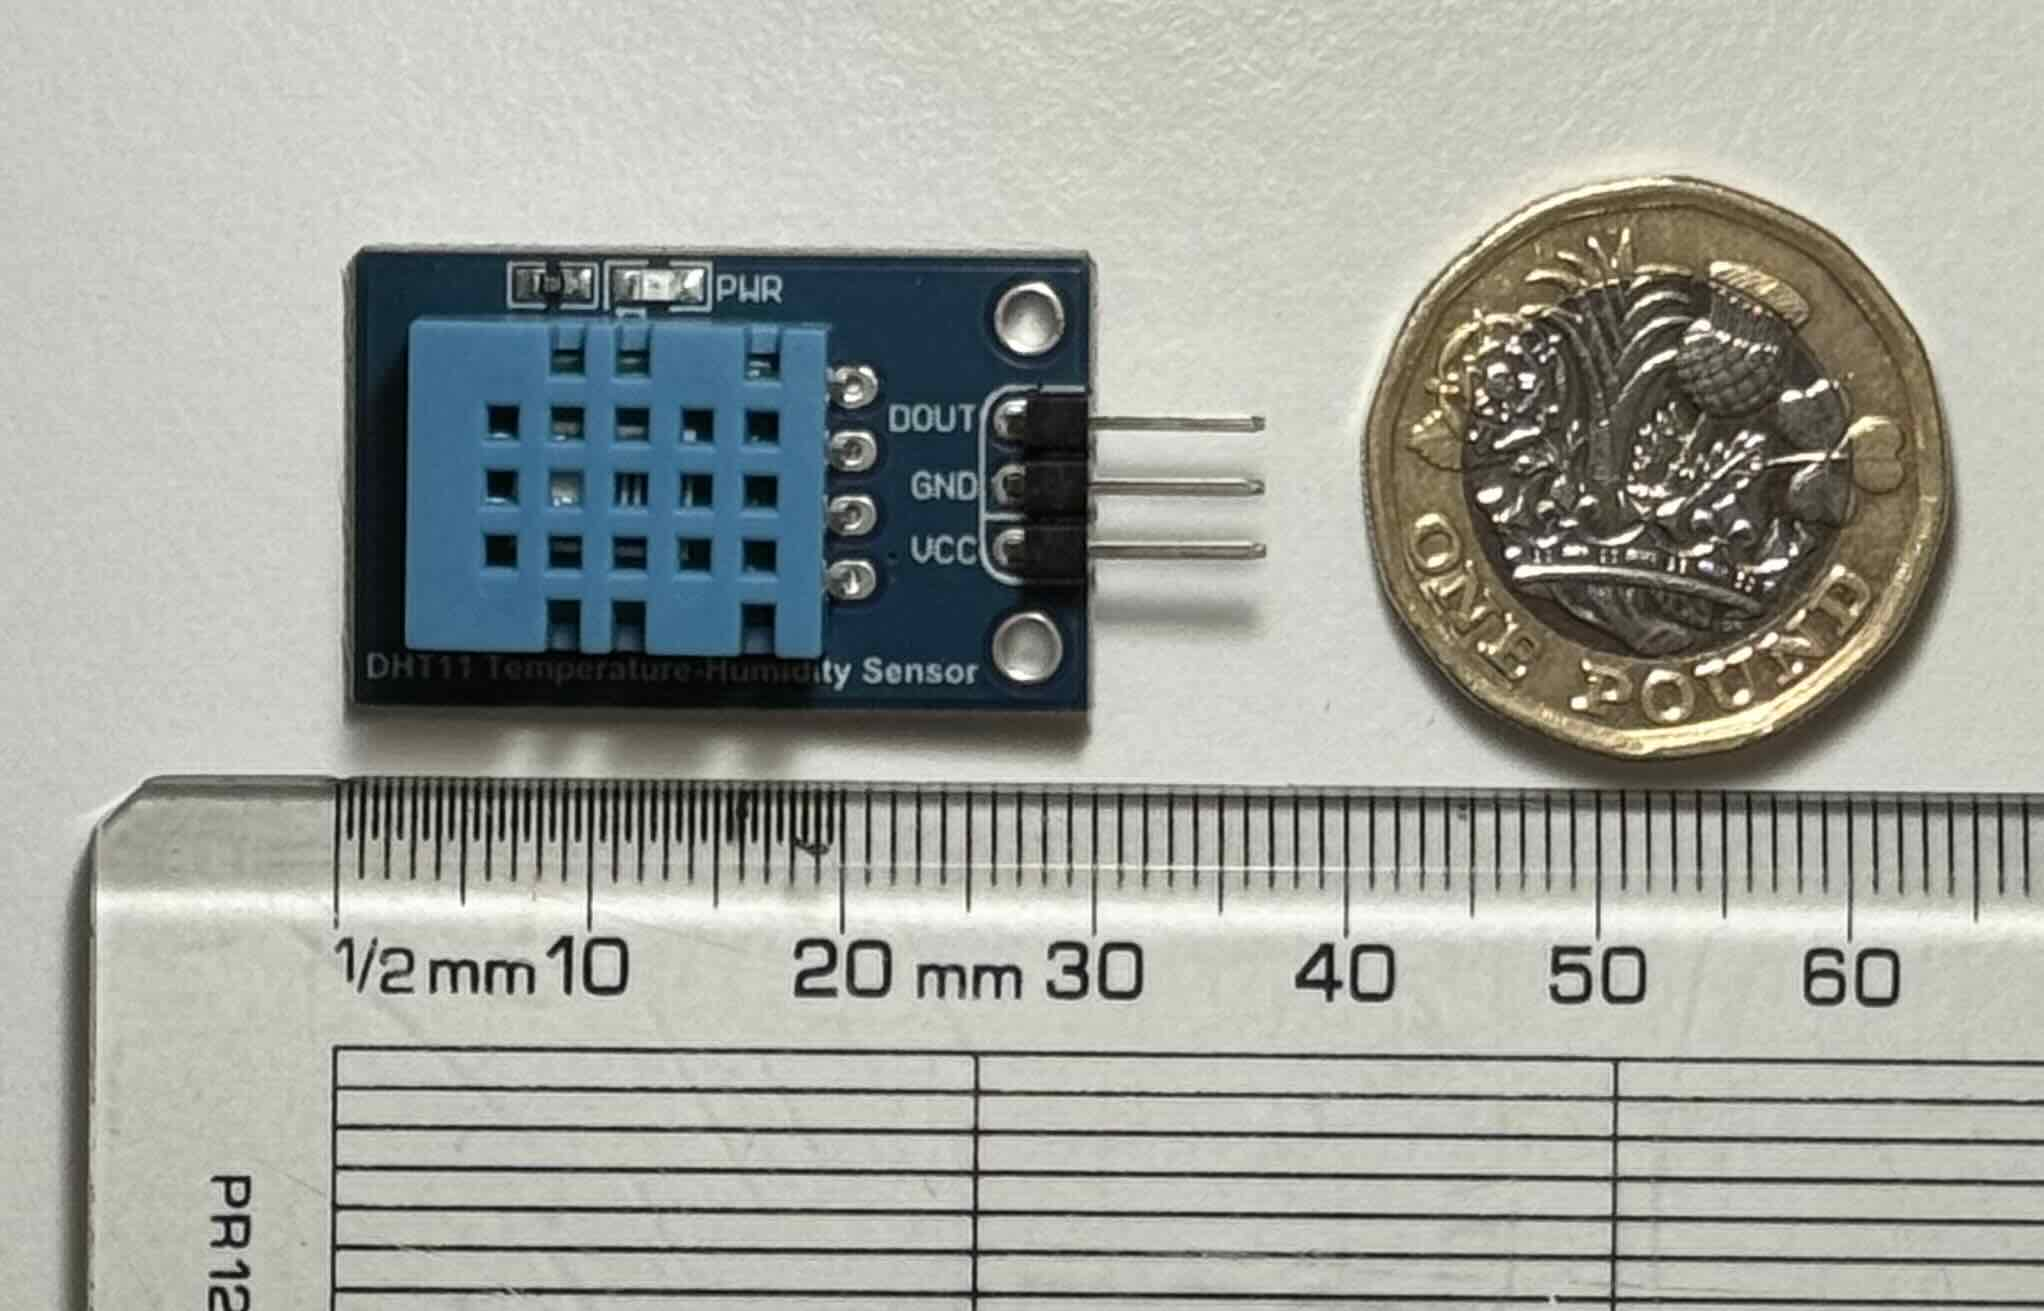
\includegraphics[width=0.8\textwidth]{contents/22-hw-design/22-fig/dht11.jpg}
    \caption{Waveshare DHT11 Temperature/Humidity sensor}
    \label{fig:dht11}
\end{figure}

\subparagraph{Soil moisture sensor}

\subparagraph{Wind speed sensor}

\paragraph{Powering the node}

To allow for continuous operation away from power sources, I set up a 5.5v
Monocrystalline Silicon Solar Panel to each of the nodes. As the output from the
solar panels was too high voltage to directly power the nodes I also installed a
solar power management module onto the Challengers. This module powers a battery
that is installed on it using a solar panel. It then is able to power the RP2040
using this battery, allowing for overnight or overcast usage of the challenger.

\paragraph{Weather proofing}

I 3D printed a water proof enclosure and a separate Stevenson weather shield for
the temperature/humidity sensor to allow for accurate outdoor readings.

\subsubsection{Programming the nodes}

On each challenger I flashed the drives with CircuitPython, an open source
interpretted language similar to Python but simplified for use in
microcontrollers.

\subsubsection{Repeater node}

To improve range I made one of the four RP2040 challengers I used act as a
repeater. This meant it did not require sensors like I used for the other two
nodes and instead it just had a solar panel and battery connected up to it. The
repeater would receive signals from the two nodes before relaying them to the
final gateway. This had the effect of significantly boosting the range.

\subsection{Gateway}

The gateway consisted of a fourth Challenger RP2040 connected to a Raspberry Pi
(TBD version). The challenger only received messages from the repeater and
then would transfer these to the Raspberry Pi. After receiving data the
Raspberry pi uploaded this to the internet.

\subsection{LoRa settings}

LoRa has many parameters that must be aligned for two devices to communicate successfully. These include:

\begin{enumerate}
  \item \textbf{Spreading factor:} 
  \item \textbf{Frequency:} Must match across devices; this project uses 868\,MHz, the UK LoRa ISM band.
  \item \textbf{Bandwidth:} Determines how wide the signal is, I am using 125\,kHz.
  \item \textbf{Coding rate:} 
  \item \textbf{Transmit power:} Affects the power and therefore range. This must be set within legal limits (e.g., 14\,dBm in the UK).
\end{enumerate}

\subsubsection{Compliance with regulatory limits on radio power}

The UK has strict regulations on the usage of radio transmitters under the Ofcom ISM band rules.
For the 868mhz band, the maximum effective radiated power that can be used is 25mW. This corresponds to a transmit power of roughly 14dB.

Additionally, the UK has rules on duty cycle rates. This is essentially how long
radio signals are permitted to be on air. For example at a spreading factor of
12 a message may take approximately 1 second to send. The duty cycle limit in
the UK is 1\%, meaning you may only transmit for 1\% of the time on a given day.
1\% of a day is 864 seconds. This means to stay in line with UK regulations only
864 messages could be sent on a given day - or roughly 1 message every 2
minutes.